\documentclass[10.5pt]{ctexart}
\usepackage{graphicx}
\usepackage{indentfirst}
\usepackage[a4paper, inner=1.5cm, outer=3cm, top=2cm, bottom=3cm, bindingoffset=1cm]{geometry}
\usepackage{xcolor}
\usepackage{array}
\usepackage{fontspec}
\usepackage{gensymb}
\usepackage{makecell}
\usepackage{pdfpages}
\usepackage{listings}
\usepackage[lofdepth,lotdepth]{subfig}
\definecolor{darkyellow}{rgb}{1,0.9,0}
\setlength{\extrarowheight}{4pt}
\begin{document}
\title{\textbf{\fontsize{15.75pt}{\baselineskip}{波形产生电路实验报告}}} % 15.75pt is 3 号 in chinese
\author{\fontsize{12pt}{\baselineskip}{数33 赵丰 2013012178}}
\maketitle
\section{\textbf{\fontsize{12pt}{\baselineskip}{正弦振荡电路:理论-仿真-实验}}}
认为在电路稳定后二极管短路了$R_4$,因为反馈回路$F=\frac{1}{3}$,故取$R_w=20k\Omega$可产生频率为$f=\frac{1}{2\pi R_1C_1}=1kHz$的正弦波。
用Spice构建文氏桥正弦波产生电路如下:\\
\itshape 
SineWaveGenerator\\
.include LM741.MOD\\
.include 1N4148.lib\\
c2 1 6 0.01u\\
r2 1 2 16k\\
r1 2 0 16k\\
c1 2 0 0.01u\\
vpps 4 0 12\\
vnps 5 0 -12\\
r3 3 0 10k\\
rw 3 7 \colorbox{darkyellow}{20k}\\
r4 6 7 10k\\
xd1 6 7 1N4148\\
xd2 7 6 1N4148\\
xLM741 2 3 4 5 6 LM741/NS\\
.tran 50u 18m\\
.end\\
\upshape
其中二极管使用了1N4148的仿真模型,运放使用了LM741的仿真模型。运行上述cir文件,产生的输出波形图如下:
\newpage
\begin{figure}[!ht]
\centering
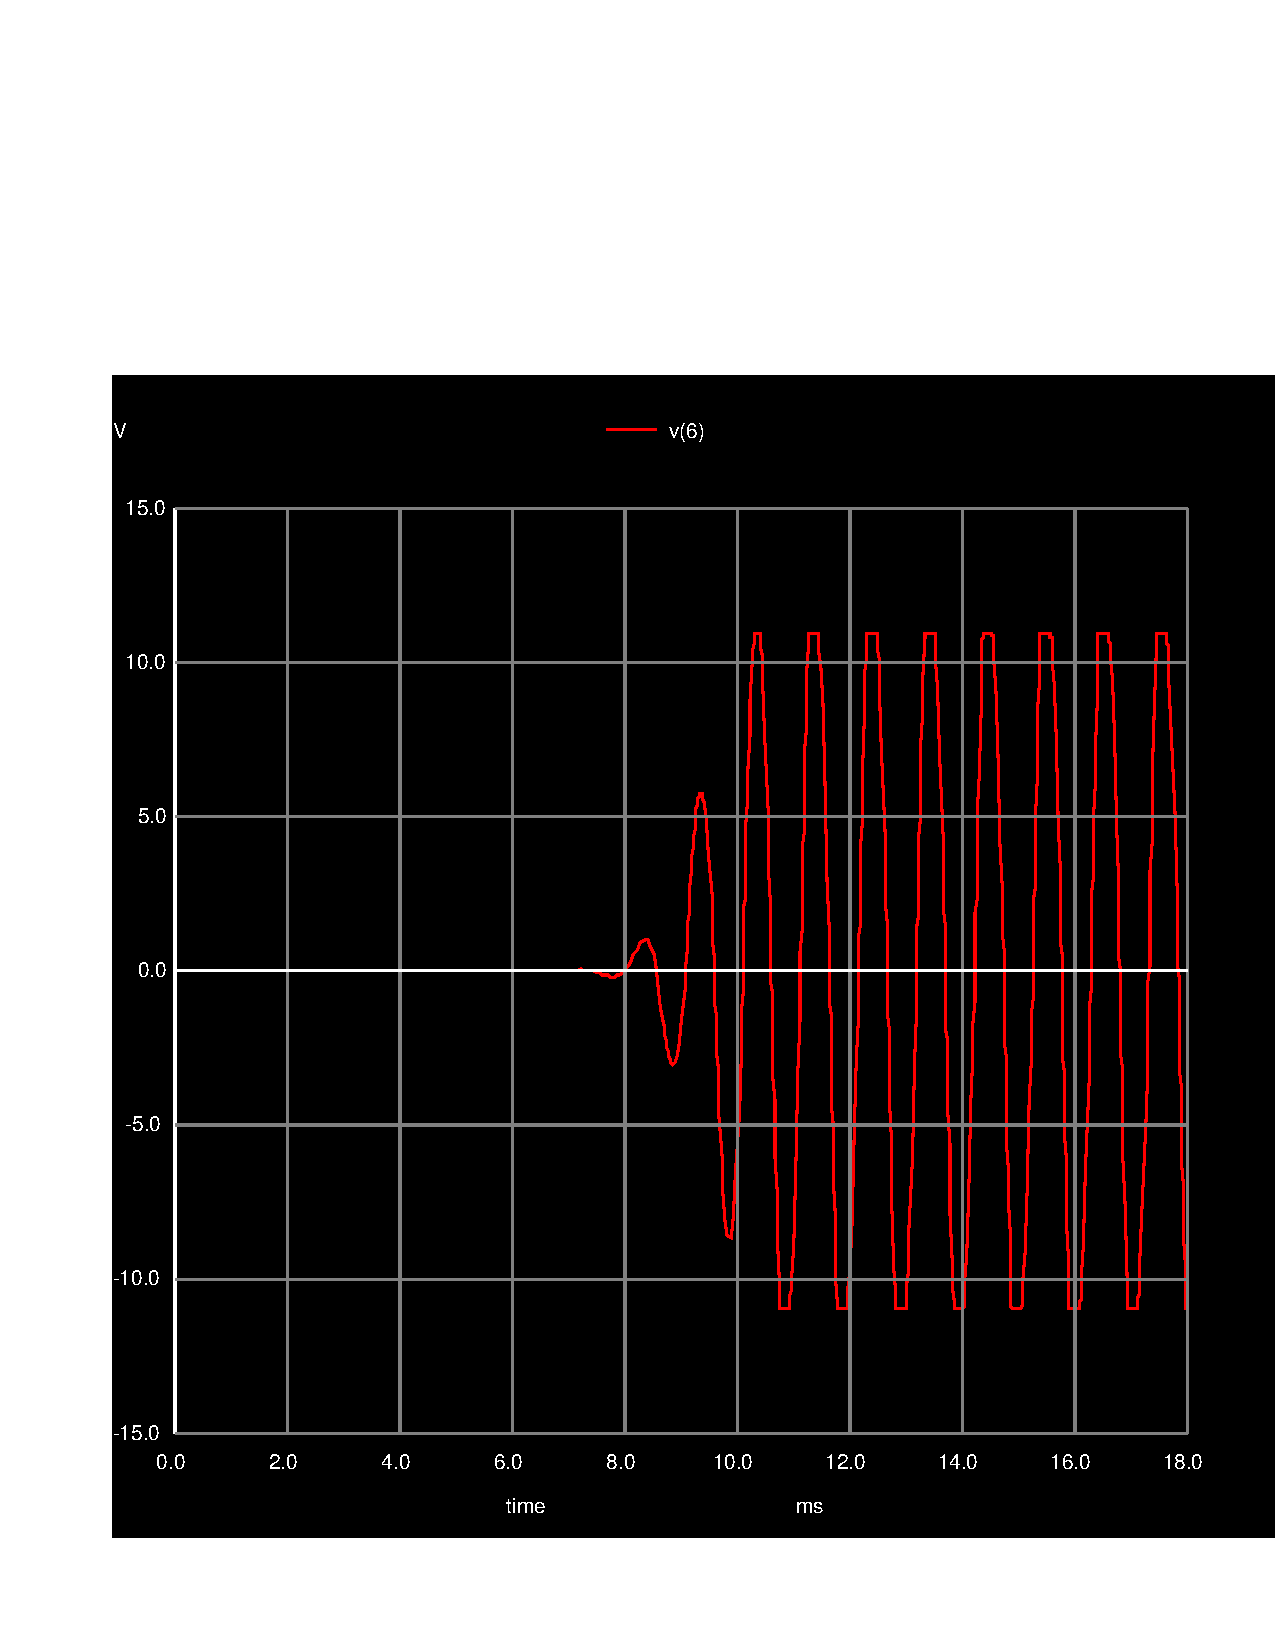
\includegraphics[width=400pt]{tranWave.pdf}
\end{figure}
实验中实际调试发现20$k\Omega$附近不能产生波形,大约在$18k\Omega$附近可以,其中$17.3k\Omega$波形较好
\section{\textbf{\fontsize{12pt}{\baselineskip}{多谐振荡电路:理论-仿真-实验}}}
由于$v_{O1}$位点接稳压二极管后接地,理想情况下$v_{O1}=\pm6V$,输出方波。前级运放是一个比较器,在后级反馈电压为$\pm3V$时跳变。因此理想情况下
$v_{O2}=\pm3V$,输出三角波,其周期为$T=2R_4 C=0.4ms$
仿真时发现LM741模型产生的结果与理论值差距较大,通过SUBCKT子电路的方式换用另一种OPAMP模型得到的结果与理论值符合较好,因原仿真cir文件内容较多,此处略去。
实验测量的截图如下所示:
\newpage
\begin{figure}[!ht]
\centering
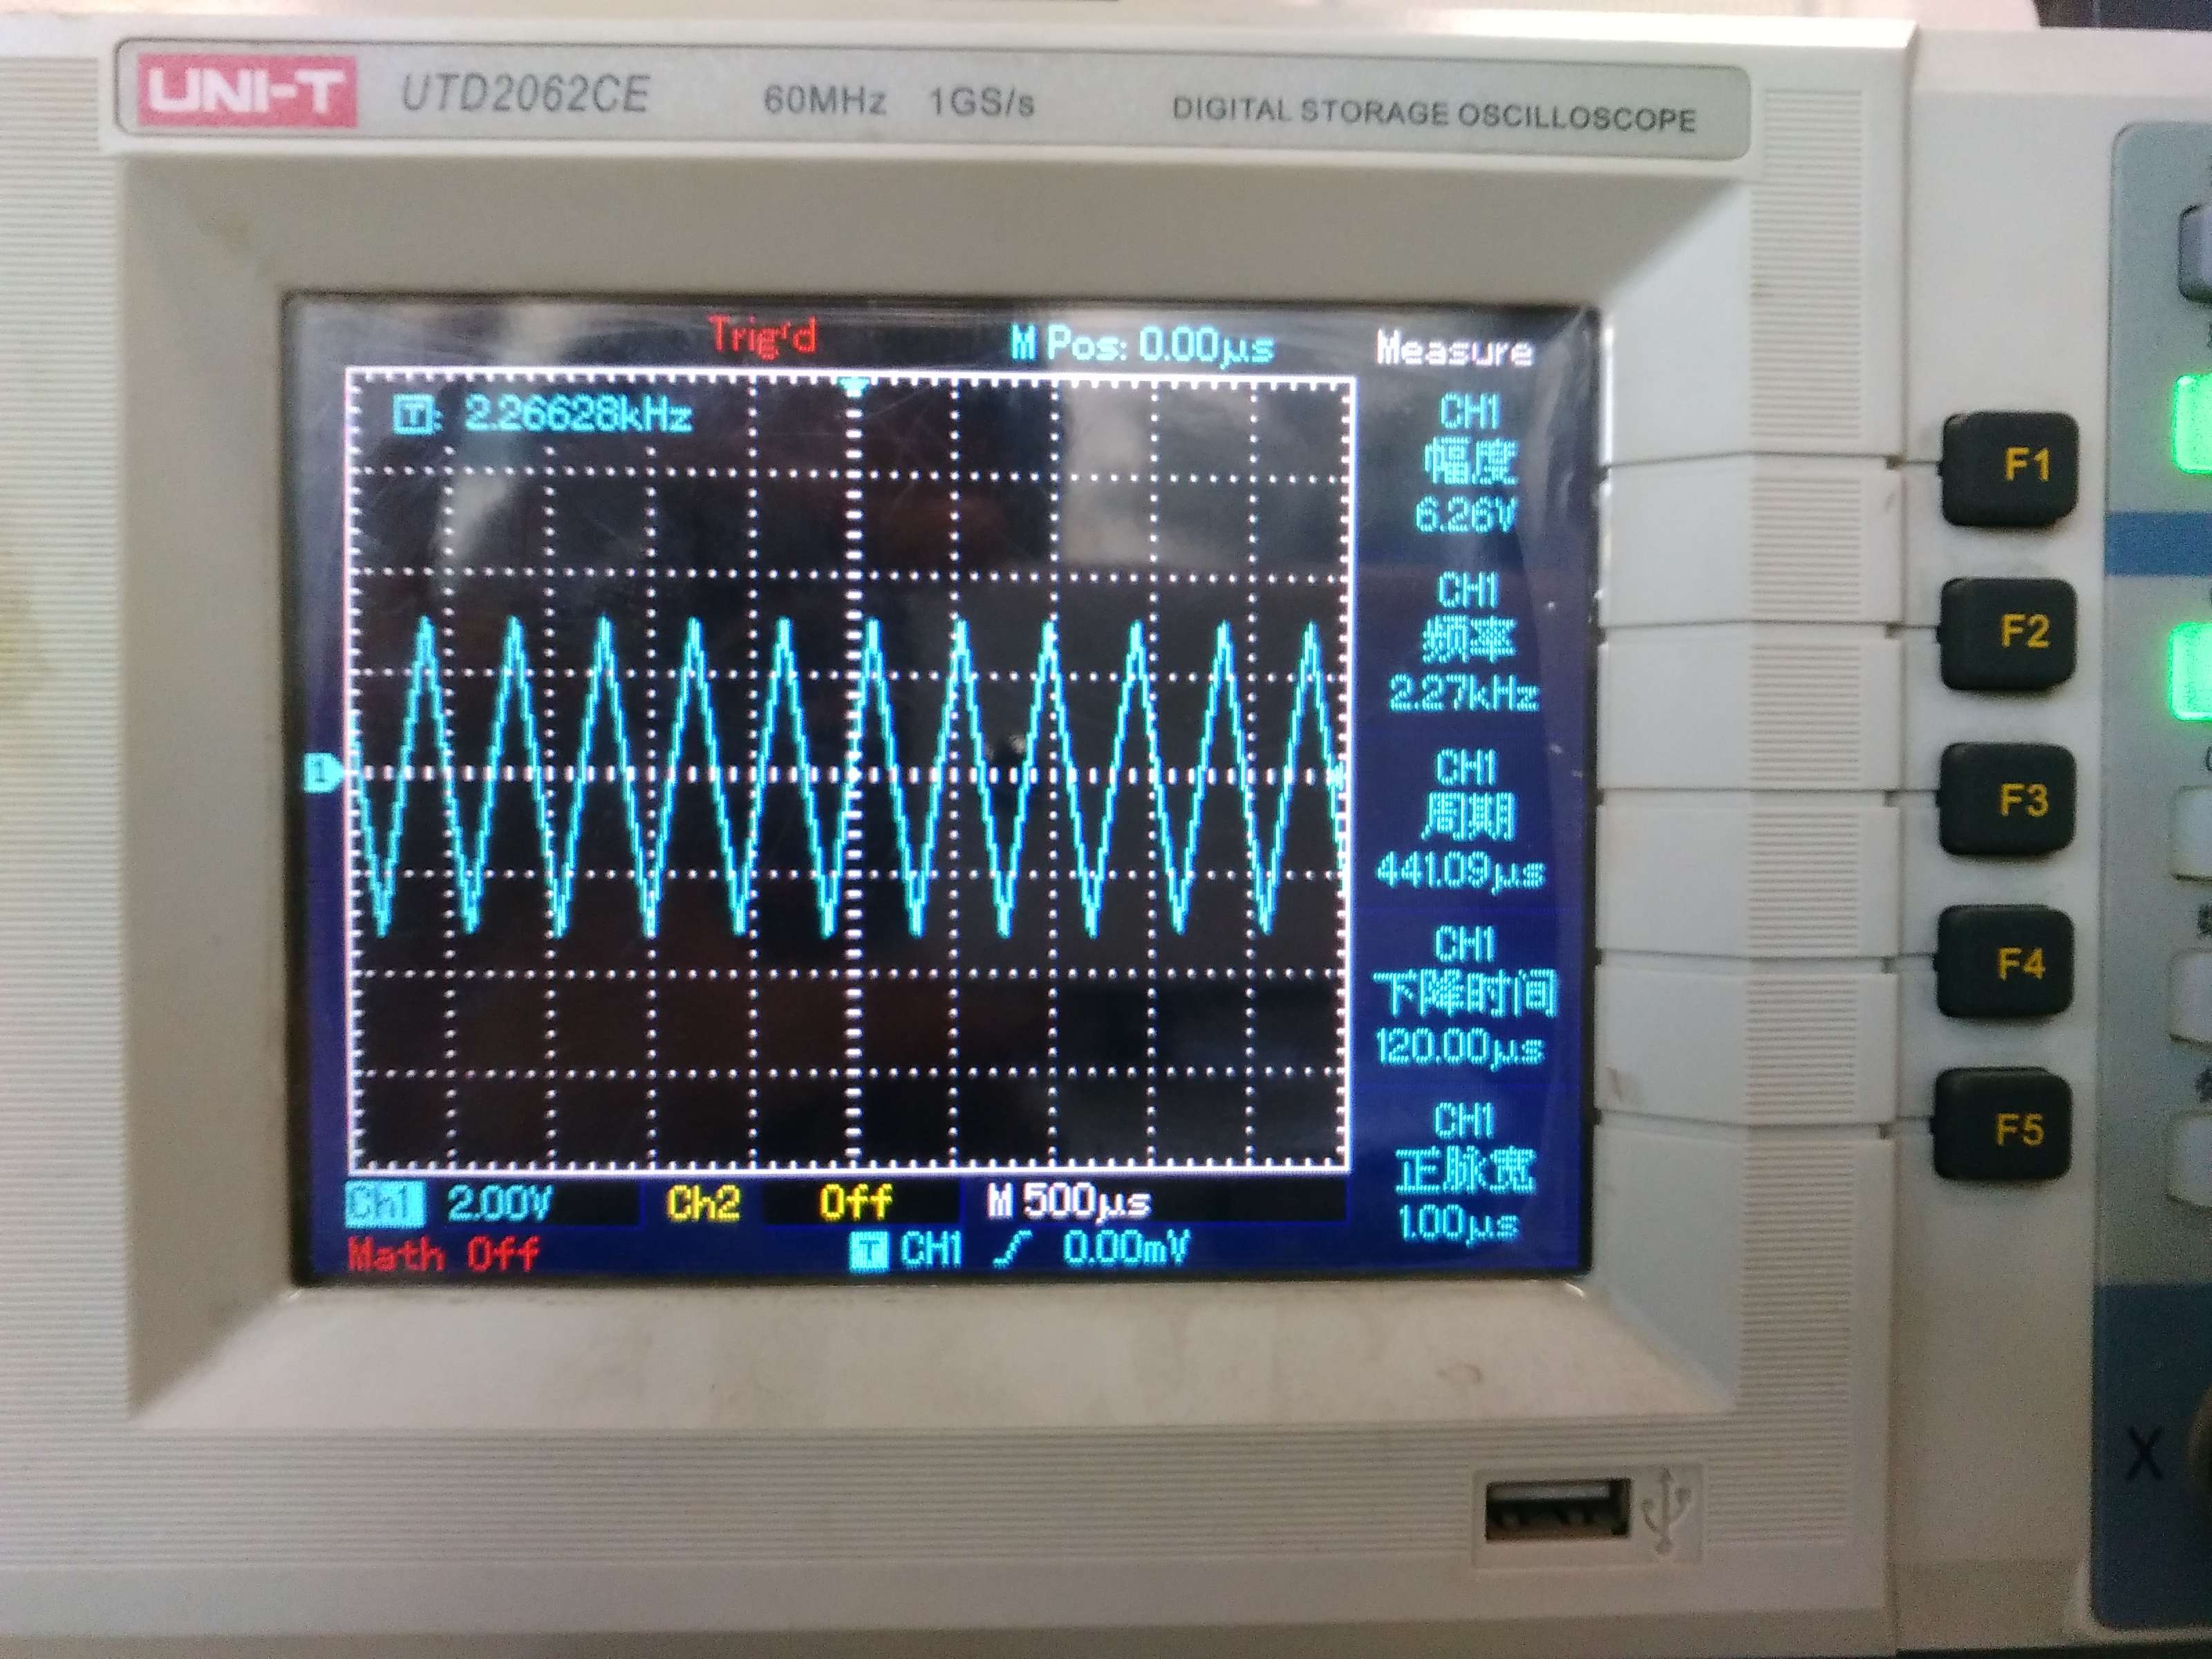
\includegraphics[width=400pt]{IMG_20161222_085444.jpg}
\end{figure}
测量结果$V_{O2}$显示三角波的Vpp=6.26V,与理论值6V相近,周期的测量值为0.44ms左右,也与理论值相差不大。$V_{O1}$处输出占空比为50\%的方波,频率与三角波相同。

将原三角波发生器中的电路中R4改为两个并联电路,其中一个并联电路为一个二极管和7.5$k\Omega$的电阻,另一个并联电路为反向的二极管和一个39$k\Omega$的电阻,实验测量中发现锯齿波电压下降段较长,调整两个二极管接入电路的极性后得到如下图所示的实验波形,锯齿波周期为576us,其中逆程为112us,正程约为逆程的4.1倍,与理论值5.2的差距在误差范围内。
\newpage
\begin{figure}[!ht]
\centering
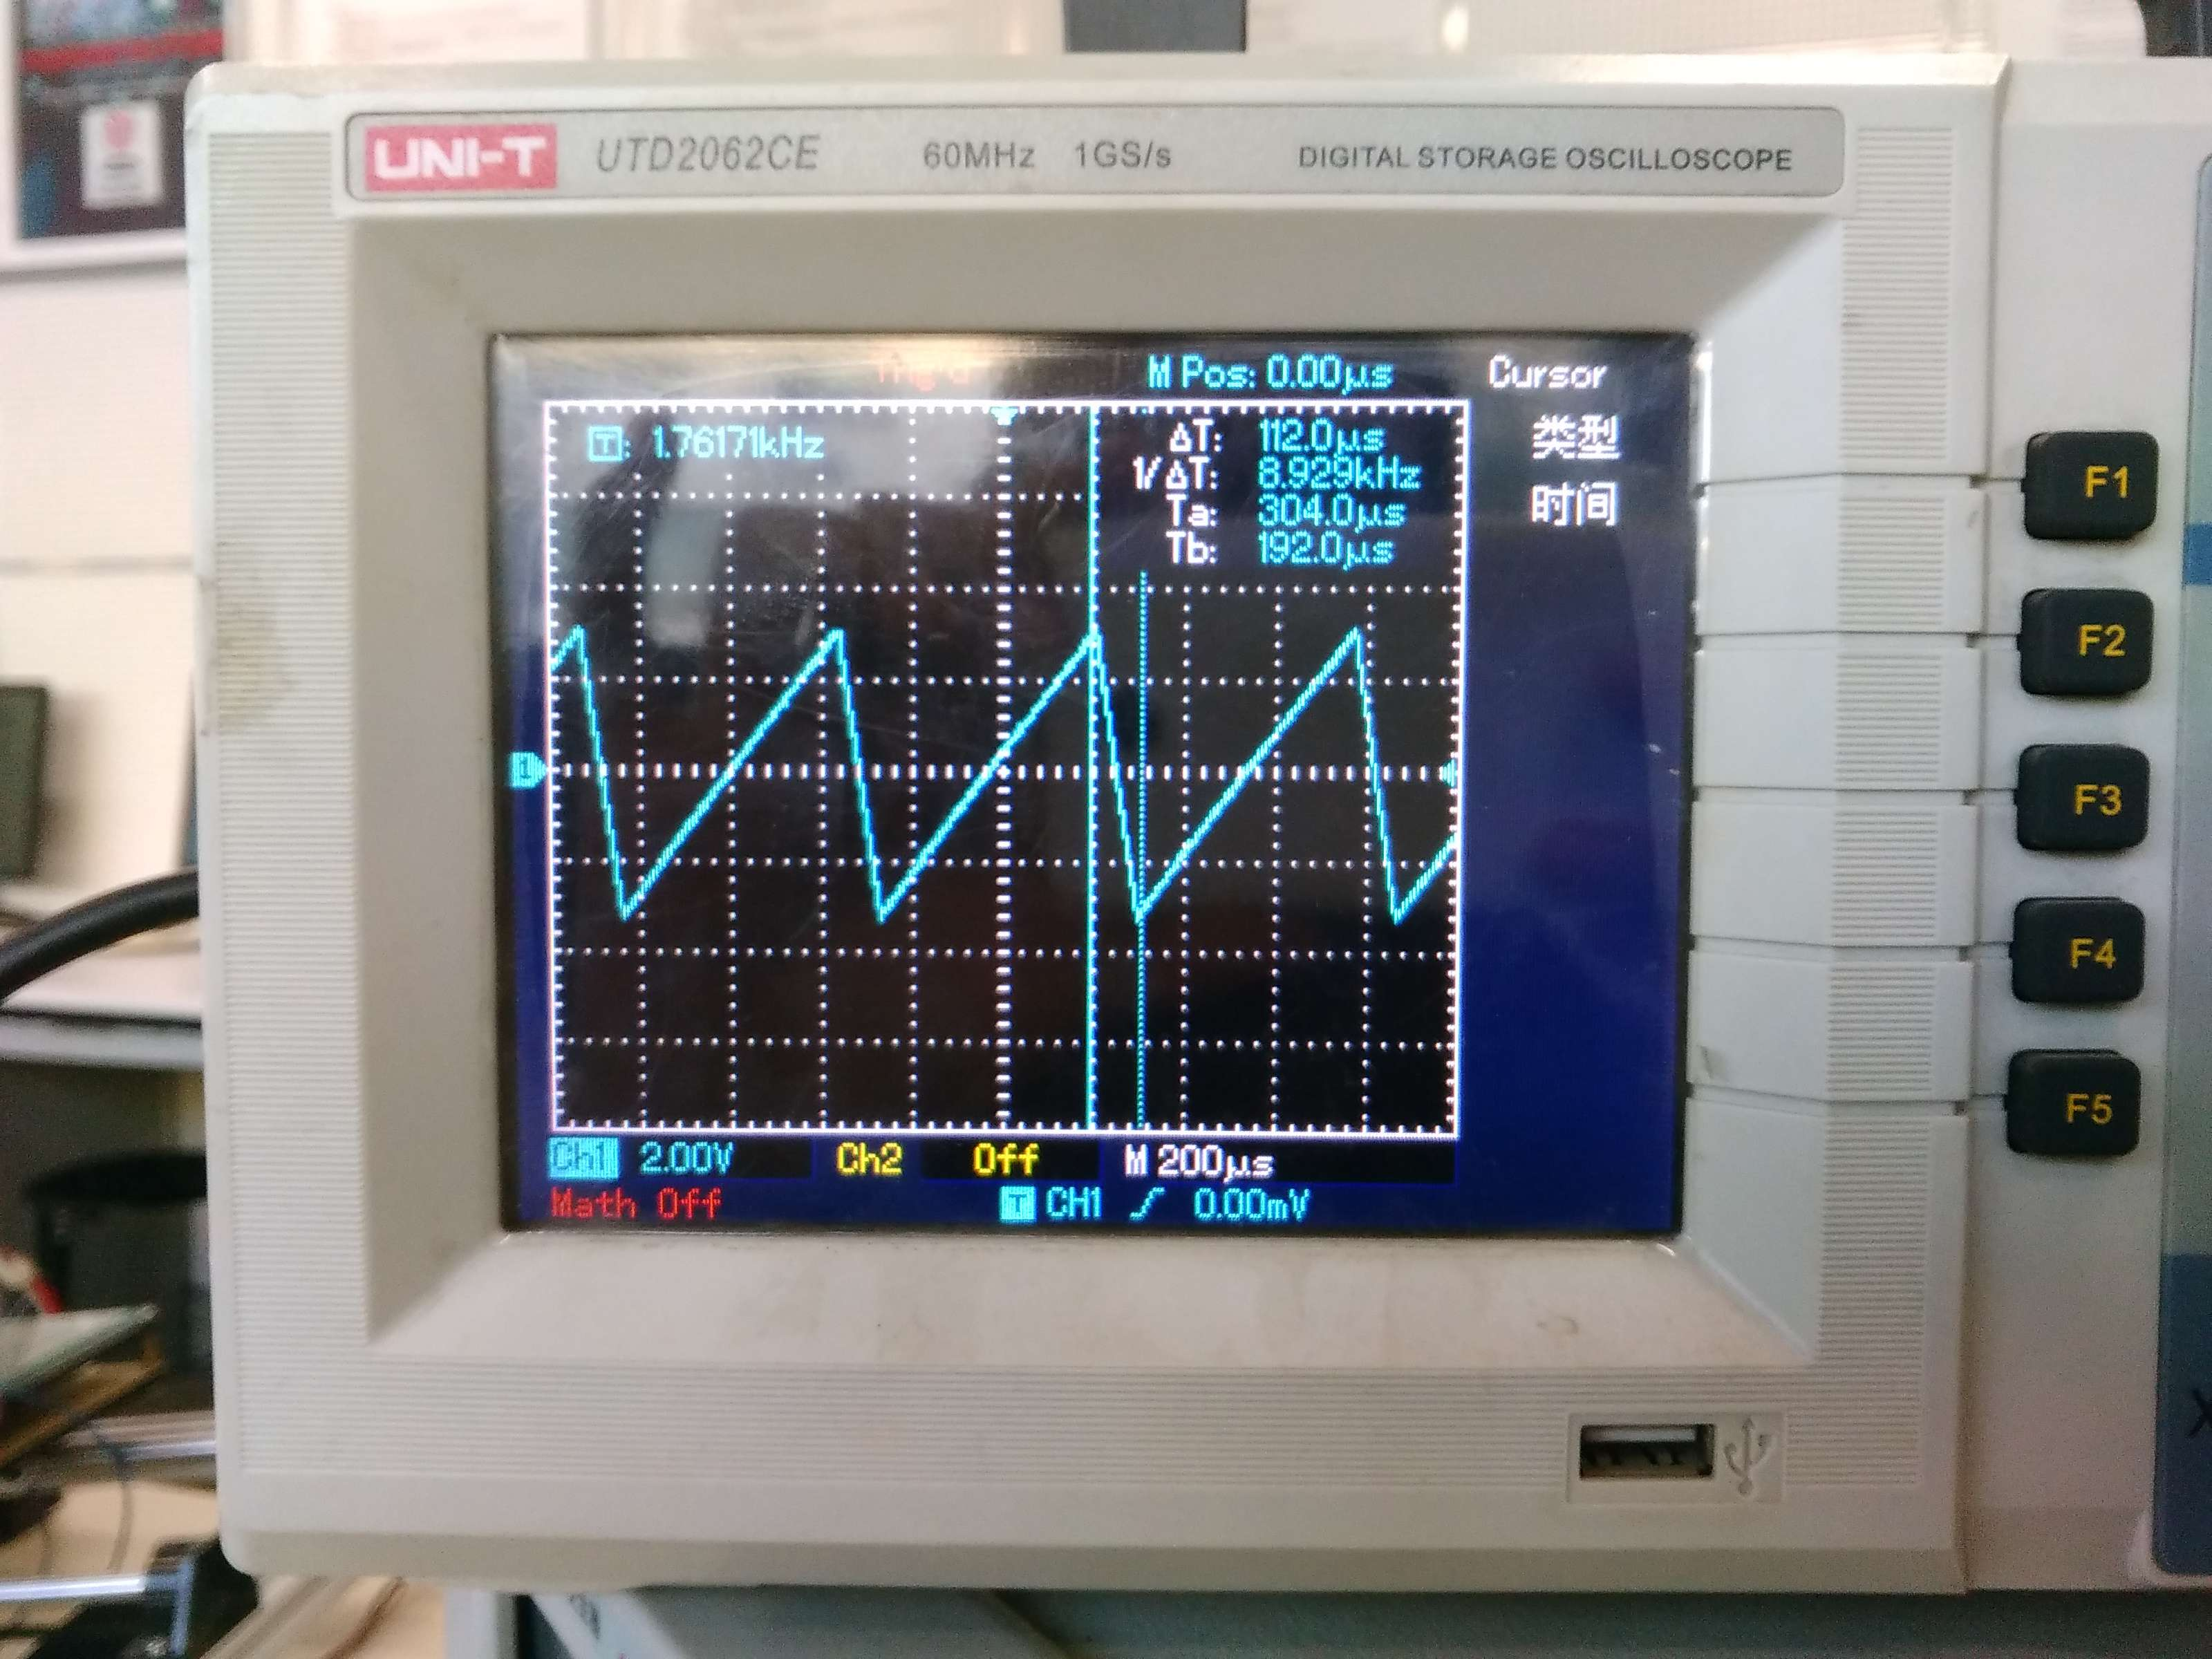
\includegraphics[width=400pt]{IMG_20161222_091521.jpg}
\end{figure}
\section{\textbf{\fontsize{12pt}{\baselineskip}{参考文献}}}
\begin{thebibliography}{}
\bibitem{Bib2}电工技术与电子技术(下册) \quad 清华大学出版社
\end{thebibliography}
\end{document}